%-------------------------------------------------------------------------
% ds-info-S1-boucles-imbriquees.tex
%-------------------------------------------------------------------------

%-------------------------------------------------------------------------
\documentclass[11pt,a4paper]{article}
%-------------------------------------------------------------------------

%-------------------------------------------------------------------------
%-------------------------------------------------------------------------
% ds-info-S1-preambule.tex
%-------------------------------------------------------------------------

%-------------------------------------------------------------------------
\usepackage{calc}
\usepackage[text={16cm,23cm},centering=true,showframe=false]{geometry}
\usepackage{fancybox,fancyvrb,fancyhdr,lastpage,lineno,import}
\usepackage{longtable,multirow}
\usepackage{xcolor,graphics,xmpmulti,pgf,pgfpages,tikz,wrapfig}
\usepackage{colortbl,color}
\usepackage{amsmath,amssymb,amsfonts}
\usepackage{hyperref,multimedia,rotating,framed,pstricks}
\usepackage{listings,index}
%
%---- pdflatex
%\usepackage[T1]{fontenc}
%\usepackage[utf8]{inputenc}
%---- xelatex
\usepackage{fontspec}
%
\usepackage[french]{minitoc}
\usepackage[french]{babel}
\usepackage[french]{nomencl}
\usepackage[framed,hyperref,standard]{ntheorem}
\usepackage{eurosym,pifont}
%-------------------------------------------------------------------------

%-------------------------------------------------------------------------
\lstset
{
language=Python,
basicstyle=\ttfamily,
identifierstyle=\ttfamily,
keywordstyle=\color{blue}\ttfamily,
commentstyle=\color{gray}\ttfamily,
stringstyle=\color{green}\ttfamily,
showstringspaces=false,
extendedchars=true,
numbers=left, 
numberstyle=\color{blue}\tiny,
frame=lines,
linewidth=0.95\textwidth,
xleftmargin=5mm
} 
%-------------------------------------------------------------------------

%-------------------------------------------------------------------------
\pgfdeclareimage[width=3cm,interpolate=true]{logo-enib}{logo-enib}
%-------------------------------------------------------------------------

%-------------------------------------------------------------------------
\pagestyle{fancy}
\fancyhead{}
\fancyhead[L]{\hspace*{-3em}\begin{minipage}{3cm}\pgfuseimage{logo-enib}\end{minipage}}
\fancyhead[C]{Informatique S1}
\fancyhead[R]{\thepage/\pageref{LastPage}}
\fancyfoot{}
\fancyfoot[L]{}
\fancyfoot[C]{}
\fancyfoot[R]{}
\setlength{\headheight}{80pt}
\setlength{\footskip}{38pt}
\renewcommand{\headrulewidth}{0pt}
\renewcommand{\footrulewidth}{0pt}
%-------------------------------------------------------------------------


%-------------------------------------------------------------------------
\def\entete{\noindent\begin{tabular}{|l|l|l|l|} 
\hline 
 & & & \\ 
\makebox[4.55cm][l]{\bsc{Nom :}} & \makebox[4.5cm][l]{\bsc{Prénom :}} & \makebox[2.5cm][l]{\bsc{Groupe :}} & \makebox[2.75cm][l]{\bsc{Question :}} \\[1mm] 
\hline 
\end{tabular}\\[1mm]
{\footnotesize \textsc{Durée : 15'\hfill Documents, calculettes, téléphones et ordinateurs interdits}}}

\def\notes{\begin{tabular}{|c|c|c|c|}  
\hline 
\makebox[0.5cm]{3} & \makebox[0.5cm]{2} & \makebox[0.5cm]{1} & \makebox[0.5cm]{0} \\  
\hline
\end{tabular}  
} 

\def\autoevaluation{$$\begin{tabular}{|c|c|c|}
\hline
\multicolumn{3}{|c|}{\textbf{Auto-évaluation}} \\
\hline
\textbf{M} & \textbf{V} & \textbf{R} \\
Méthode(s) & Vérification(s) & Résultat(s) \\
\notes & \notes & \notes \\[1mm]
\hline
\end{tabular}$$ $$ $$}

\def\reponse{\mbox{}\hfill \fbox{\huge Réponse page suivante}}
%-------------------------------------------------------------------------

%-------------------------------------------------------------------------
\tikzset{
xmin/.store in=\xmin, xmin/.default=-3, xmin=-3,
xmax/.store in=\xmax, xmax/.default=3,  xmax=3,
ymin/.store in=\ymin, ymin/.default=-3, ymin=-3,
ymax/.store in=\ymax, ymax/.default=3,  ymax=3,
}

\newcommand{\grille}{\draw[color=lightgray] (\xmin,\ymin) grid (\xmax,\ymax);}

\newcommand{\axes}{
	\draw[->] (\xmin,0) -- (\xmax,0);
	\draw[->] (0,\ymin) -- (0,\ymax);
}

\newcommand{\fenetre}{\clip (\xmin,\ymin) rectangle (\xmax,\ymax);}
%-------------------------------------------------------------------------

%-------------------------------------------------------------------------
\def\ga{\textsc{ga}}   
\def\bu{\textsc{bu}} 
\def\zo{\textsc{zo}} 
\def\meu{\textsc{meu}} 
%-------------------------------------------------------------------------


%-------------------------------------------------------------------------
\input{sigle}
%-------------------------------------------------------------------------

\graphicspath{{../../fig/}}



%-------------------------------------------------------------------------

%-------------------------------------------------------------------------
\begin{document}
%-------------------------------------------------------------------------
\entete

\autoevaluation


$$\mbox{\textbf{\large Motifs géométriques}}$$


\paragraph{Questions :} 
En utilisant les instructions de la tortue \logo{}
(module \texttt{turtle}), écrire un algorithme qui dessine un motif géométrique
composé de $(n\times m)$ pavés élémentaires disposés régulièrement sur une grille
ou disposés en quinconce sur la grille.
\vspace*{3mm}

\begin{minipage}[t]{7cm}
\begin{enumerate}
\item \begin{minipage}{1.75cm}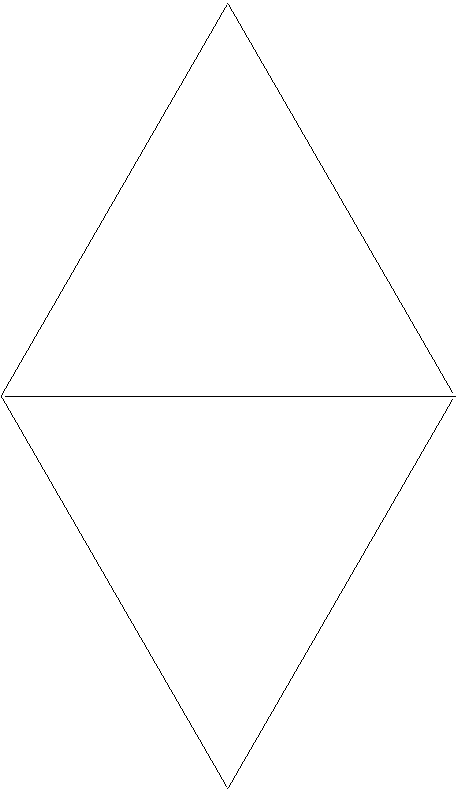
\includegraphics[height=0.75cm]{losange-2.pdf}\end{minipage} alignés
\item \begin{minipage}{1.75cm}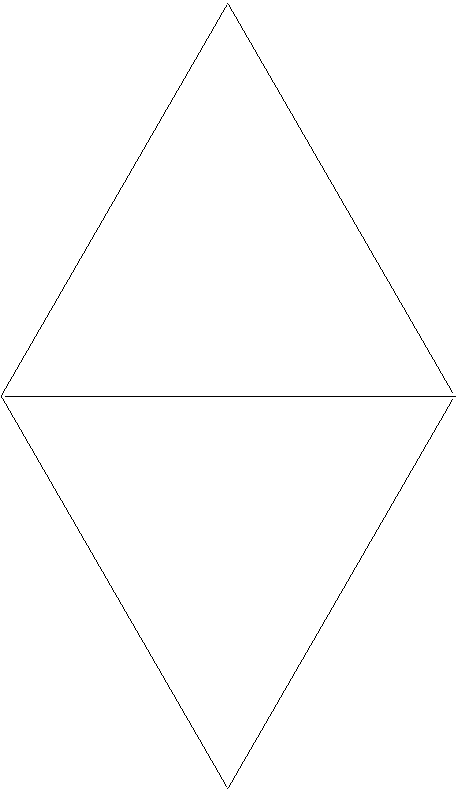
\includegraphics[height=0.75cm]{losange-2.pdf}\end{minipage} en quinconce
\item \begin{minipage}{1.75cm}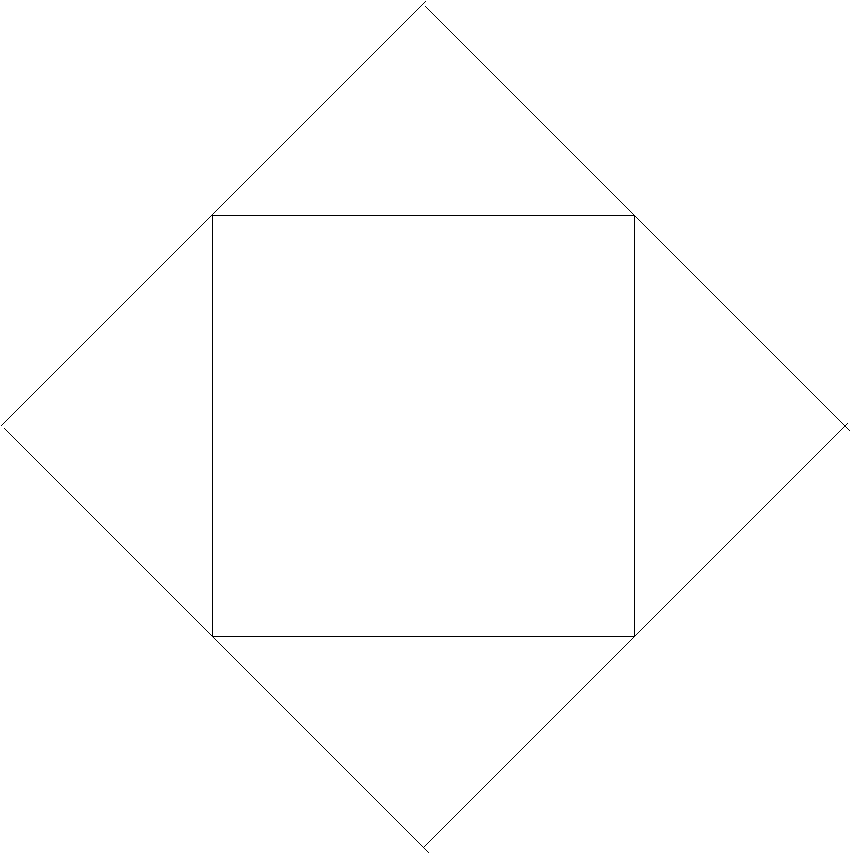
\includegraphics[height=0.75cm]{carre-2.pdf}\end{minipage} alignés
\item \begin{minipage}{1.75cm}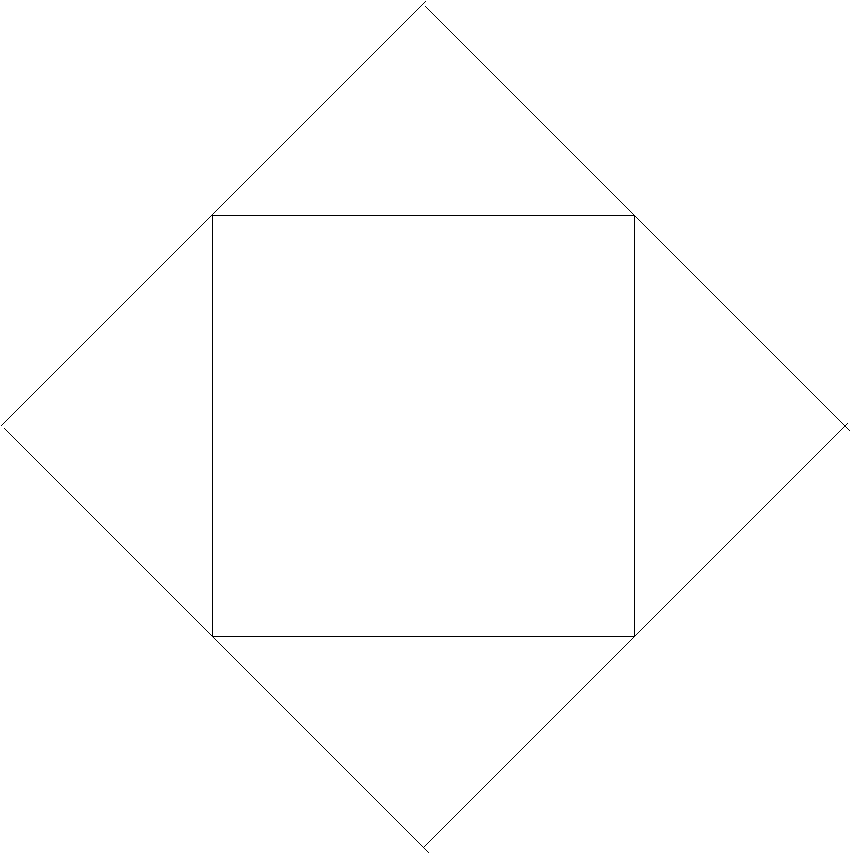
\includegraphics[height=0.75cm]{carre-2.pdf}\end{minipage} en quinconce
\item \begin{minipage}{1.75cm}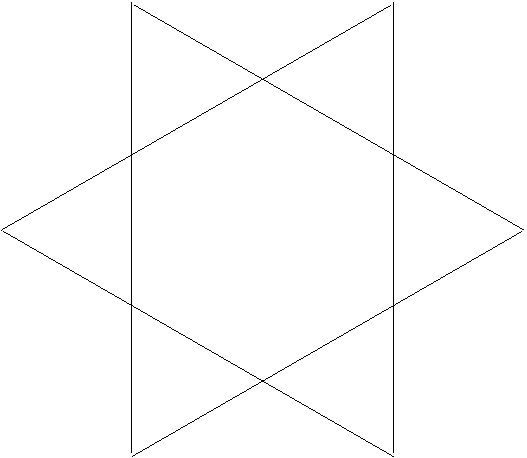
\includegraphics[height=0.75cm]{etoile-2.pdf}\end{minipage} alignés
\item \begin{minipage}{1.75cm}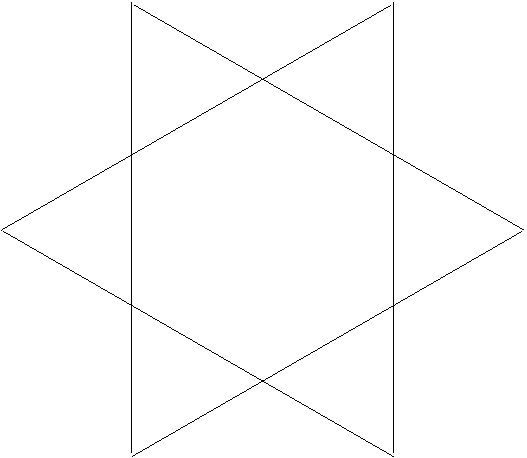
\includegraphics[height=0.75cm]{etoile-2.pdf}\end{minipage} en quinconce
\item \begin{minipage}{1.75cm}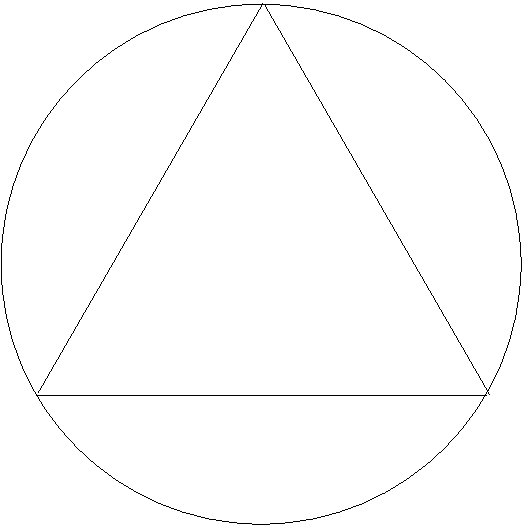
\includegraphics[height=0.75cm]{cercle-2.pdf}\end{minipage} alignés
\item \begin{minipage}{1.75cm}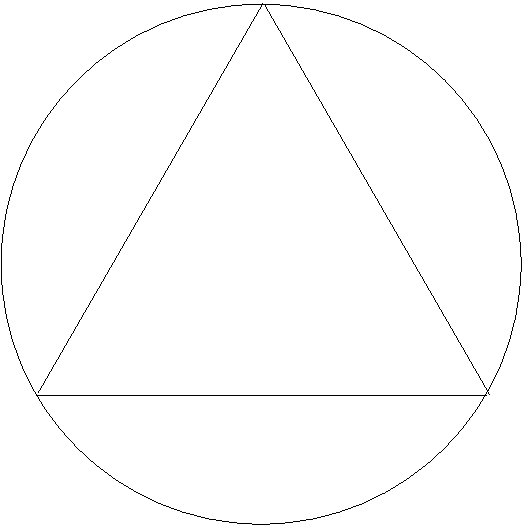
\includegraphics[height=0.75cm]{cercle-2.pdf}\end{minipage} en quinconce
\item \begin{minipage}{1.75cm}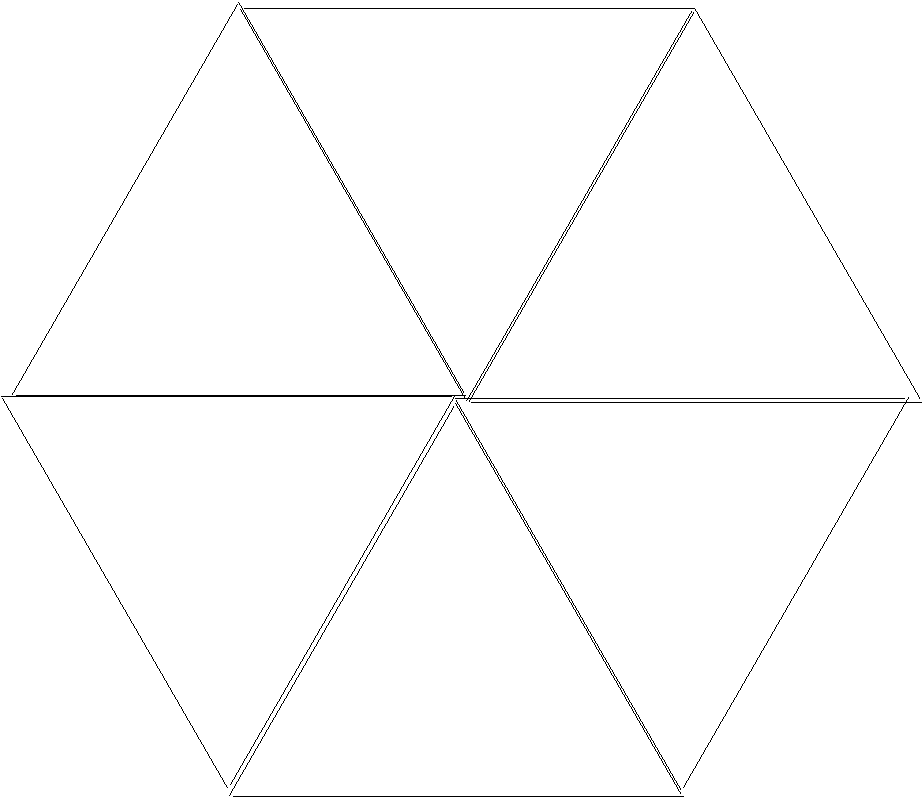
\includegraphics[height=0.75cm]{hexagone-2.pdf}\end{minipage} alignés
\item \begin{minipage}{1.75cm}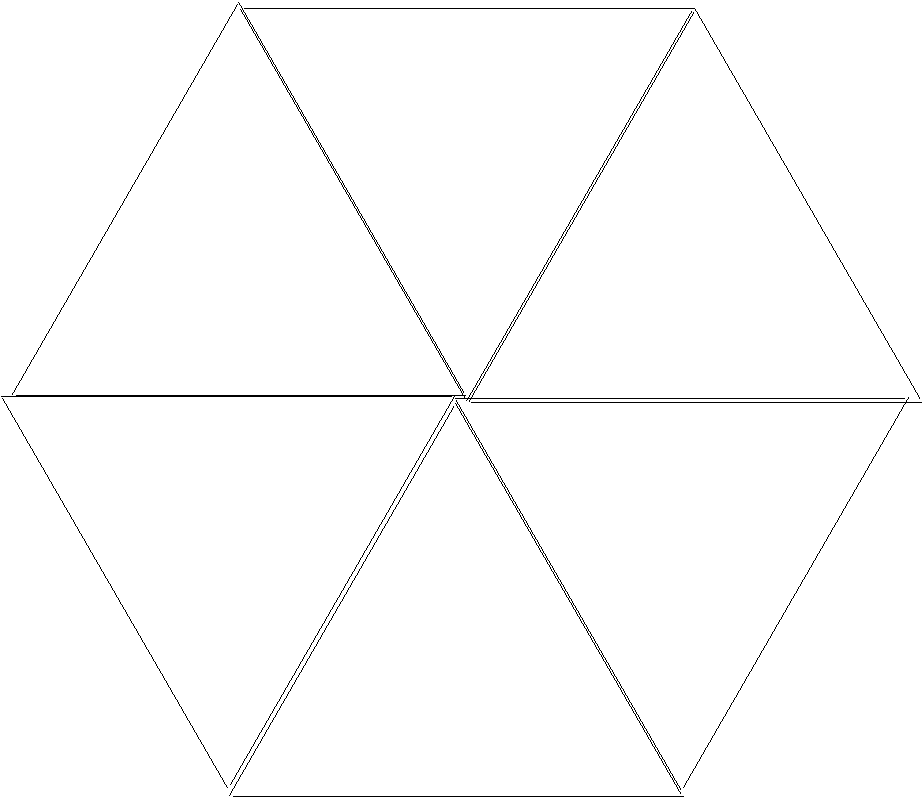
\includegraphics[height=0.75cm]{hexagone-2.pdf}\end{minipage} en quinconce
\item \begin{minipage}{1.75cm}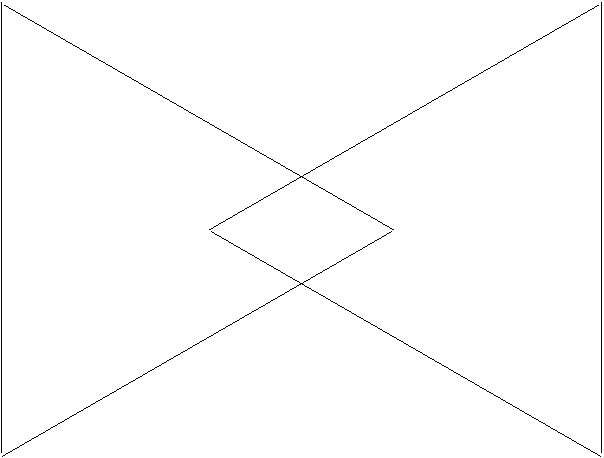
\includegraphics[height=0.75cm]{triangle-2.pdf}\end{minipage} alignés
\item \begin{minipage}{1.75cm}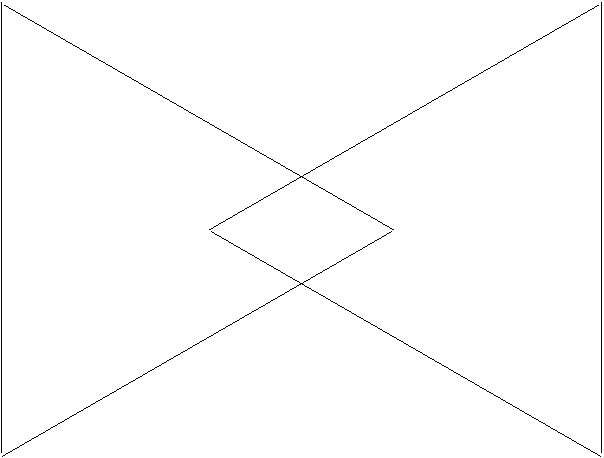
\includegraphics[height=0.75cm]{triangle-2.pdf}\end{minipage} en quinconce
\end{enumerate}
\end{minipage}
\hfill
\begin{minipage}[t]{7cm}
\begin{enumerate}\setcounter{enumi}{12}
\item \begin{minipage}{1.75cm}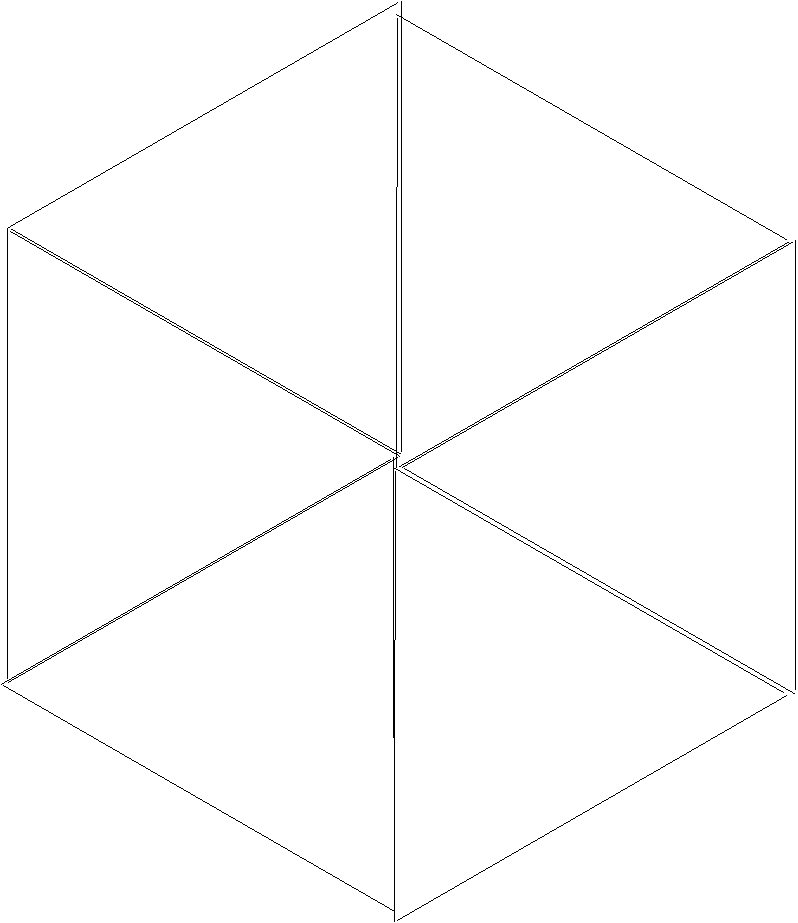
\includegraphics[height=0.75cm]{hexagone-1.pdf}\end{minipage} alignés
\item \begin{minipage}{1.75cm}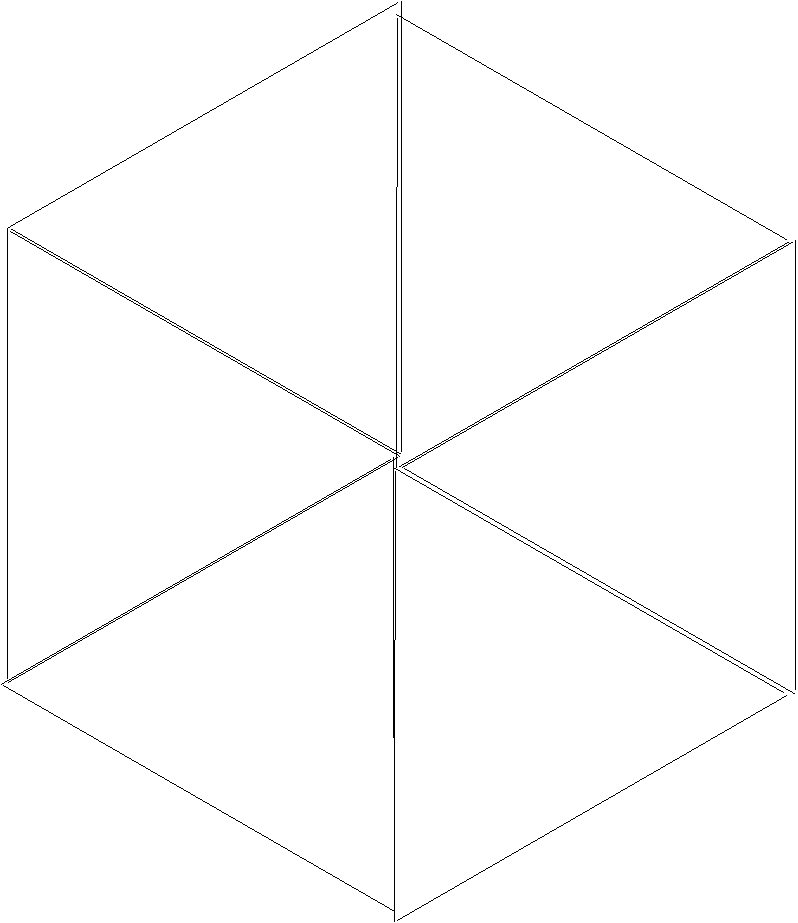
\includegraphics[height=0.75cm]{hexagone-1.pdf}\end{minipage} en quinconce
\item \begin{minipage}{1.75cm}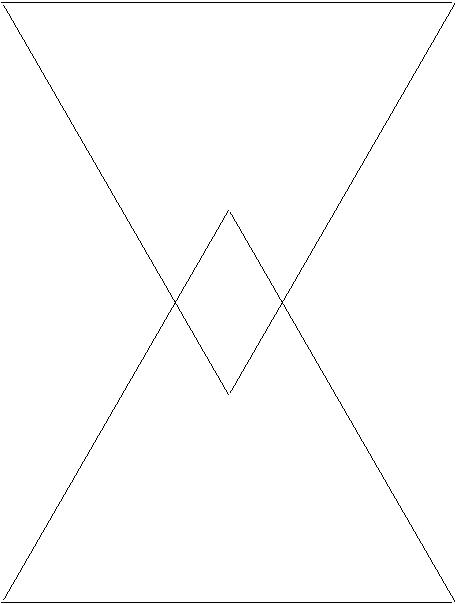
\includegraphics[height=0.75cm]{triangle-1.pdf}\end{minipage} alignés
\item \begin{minipage}{1.75cm}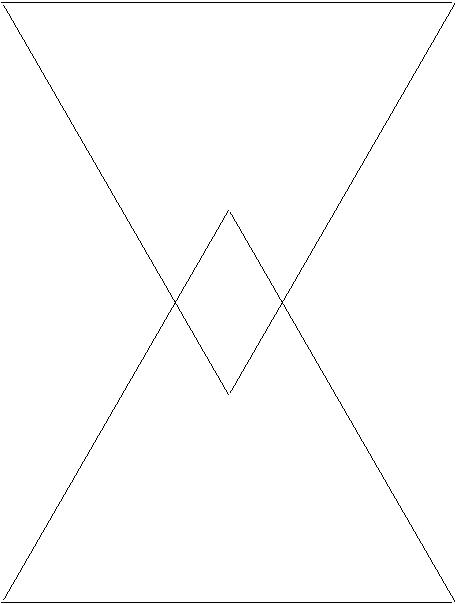
\includegraphics[height=0.75cm]{triangle-1.pdf}\end{minipage} en quinconce
\item \begin{minipage}{1.75cm}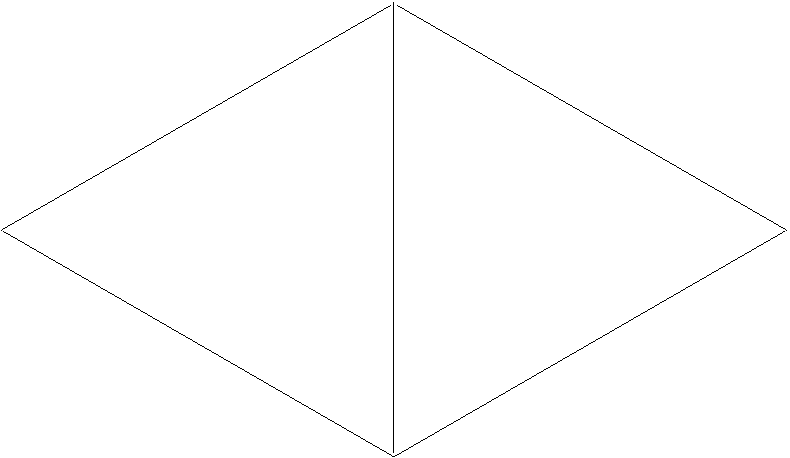
\includegraphics[height=0.75cm]{losange-1.pdf}\end{minipage} alignés
\item \begin{minipage}{1.75cm}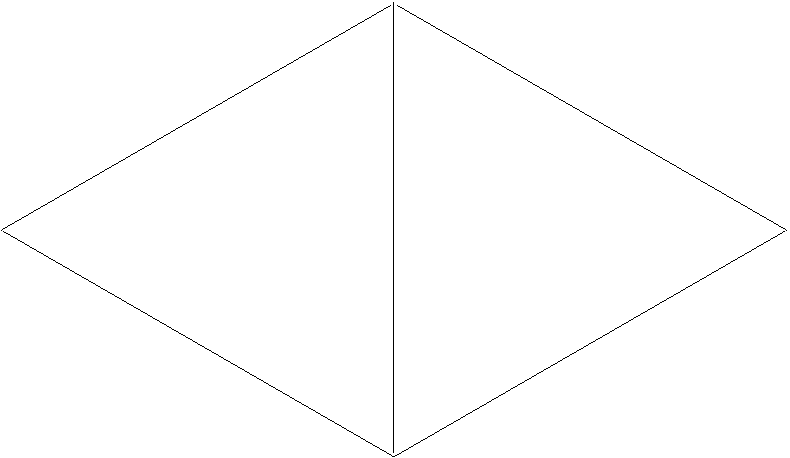
\includegraphics[height=0.75cm]{losange-1.pdf}\end{minipage} en quinconce
\item \begin{minipage}{1.75cm}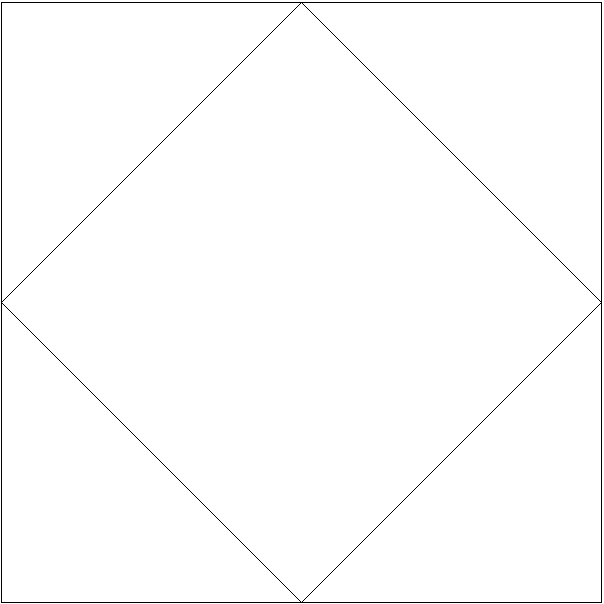
\includegraphics[height=0.75cm]{carre-1.pdf}\end{minipage} alignés
\item \begin{minipage}{1.75cm}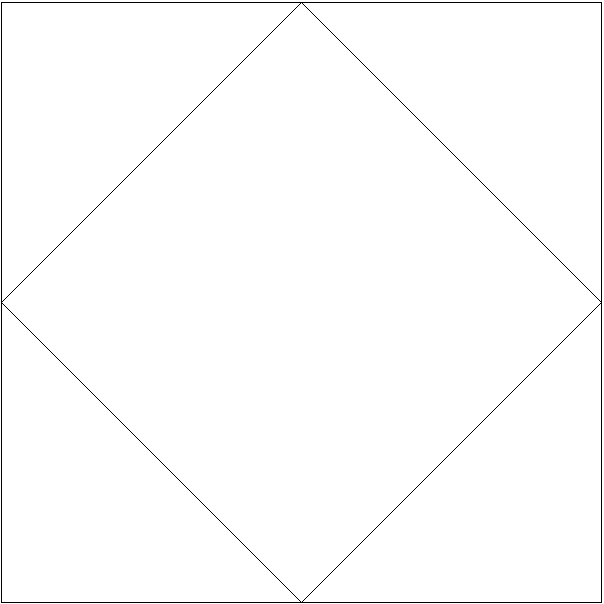
\includegraphics[height=0.75cm]{carre-1.pdf}\end{minipage} en quinconce
\item \begin{minipage}{1.75cm}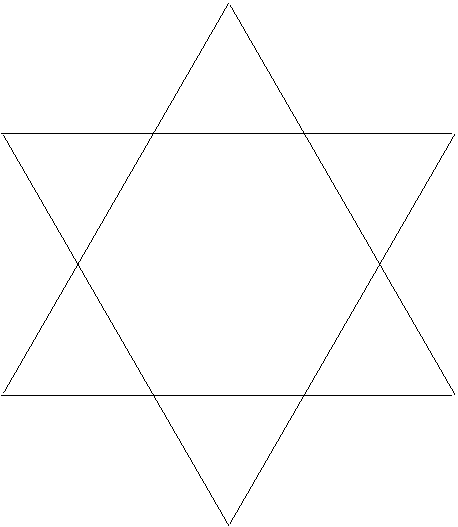
\includegraphics[height=0.75cm]{etoile-1.pdf}\end{minipage} alignés
\item \begin{minipage}{1.75cm}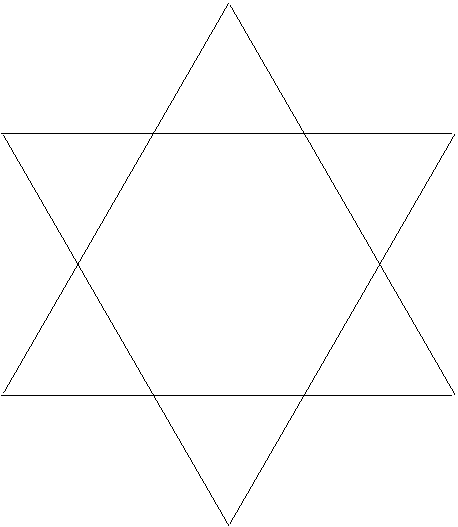
\includegraphics[height=0.75cm]{etoile-1.pdf}\end{minipage} en quinconce
\item \begin{minipage}{1.75cm}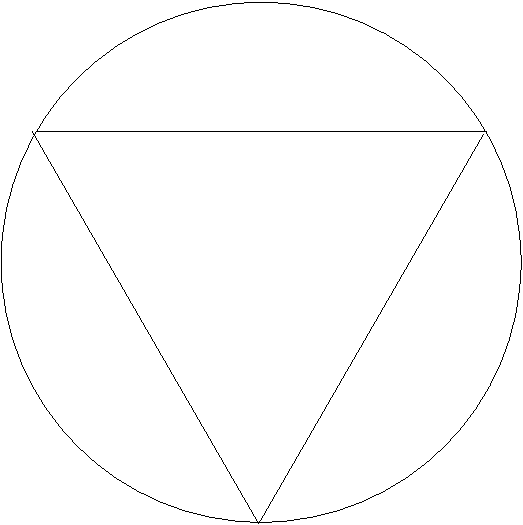
\includegraphics[height=0.75cm]{cercle-1.pdf}\end{minipage} alignés
\item \begin{minipage}{1.75cm}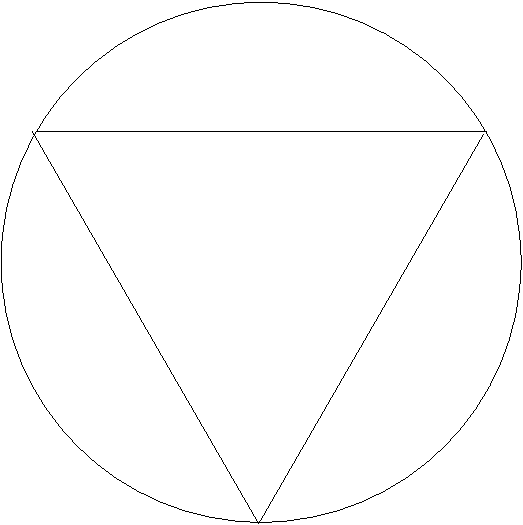
\includegraphics[height=0.75cm]{cercle-1.pdf}\end{minipage} en quinconce
\end{enumerate}
\end{minipage}
%-------------------------------------------------------------------------
\null\vfill

$$\reponse$$
%-------------------------------------------------------------------------
\paragraph{Réponse :}\mbox{}

\noindent\framebox[\textwidth]{$\rule{0cm}{0.96\textheight}$}



%-------------------------------------------------------------------------
\end{document}
%-------------------------------------------------------------------------
